\documentclass[parskip=half]{scrartcl}
% ------------------------------------------------------------------------------
% LaTeX-Grundkonfiguration von Stefan Rothe
% ------------------------------------------------------------------------------

% 1 Konfiguration der Schriftarten
% --------------------------------
% um \ifXeTeX verwenden zu können
\usepackage{iftex}

\ifXeTeX
  % Setze PDF-Version auf 1.7
  \special{pdf:minorversion 7}

  % 1.1 Konfiguration der Schriftarten für XeTeX (empfohlen)
  % ----------------------------------------------------------
  \usepackage{fontspec}

  \IfFontExistsTF{Helvetica}{\setmainfont{Helvetica}}{%
    \IfFontExistsTF{Arial}{\setmainfont{Arial}}{}%
  }

  \IfFontExistsTF{Helvetica}{\setsansfont{Helvetica}}{%
    \IfFontExistsTF{Arial}{\setsansfont{Arial}}{}%
  }

  \IfFontExistsTF{Menlo}{\setmonofont[SizeFeatures={Size=10}]{Menlo}}{%
    \IfFontExistsTF{Courier New}{\setmonofont[SizeFeatures={Size=10}]{Courier New}}{}%
  }
\else
  % Setze PDF-Version auf 1.7
  \pdfminorversion=7

  % 1.2 Konfiguration der Schriftarten für PdfTeX
  % -----------------------------------------------

  % Unterstützung von UTF-8 (Unicode)
  \usepackage[utf8]{inputenc}

  % Unterstützung der modernen Zeichencodierung
  \usepackage[T1]{fontenc}

  % Moderne Schriftart verwenden
  \usepackage{lmodern}

  % Schriftart Helvetica verwenden
  \usepackage{helvet}

  % serifenfreie Schriftvariante verwenden
  \renewcommand{\familydefault}{\sfdefault}
\fi

% 2 wichtige Pakete laden und konfigurieren
% -----------------------------------------

% sprachspezifische Anpassungen
\usepackage[ngerman]{babel}

% Absatzabstände kontrollieren für nicht-KOMA-Klassen
\makeatletter
\@ifclassloaded{scrartcl}{}{\usepackage{parskip}}
\makeatother

% Aufzählungen
\usepackage{enumitem}

% mehrere Spalten
\usepackage{multicol}

% Rahmen
\usepackage{mdframed}

% Tabellen
\usepackage{booktabs}
\usepackage{tabularx}

% Grafiken (JPG, PNG, PDF)
\usepackage{graphicx}

% Links
\usepackage{hyperref}
\hypersetup{colorlinks=true,urlcolor=blue,linkcolor=black}

% Einbinden von Quellcode
\usepackage{listings}
\lstdefinestyle{mystyle}{
  basicstyle=\ttfamily,
  numberstyle=\scriptsize\color{black!70},
  numbers=left,
  numbersep=0.75cm
}
\lstset{style=mystyle}

% 3 Mathematik
% ------------

% 3.1 Zahlen und Einheiten schön darstellen
% -----------------------------------------
\usepackage{siunitx}
\sisetup{%
  mode=match,
  exponent-product=\cdot,
  group-digits=integer,
  group-separator={\text{\textquotesingle}}
}

% 3.2 AMS-Mathematik
% ------------------

\usepackage[fleqn]{amsmath}
\usepackage{amssymb}

% 3.3 Vektoren
% ------------
\usepackage[b]{esvect}

\makeatletter
% Koordinatenschreibweise für 2D-Punkte
\NewDocumentCommand\pxy@internal{mmm}{\mathopen{}\left(#1/#2\right)\mathclose{}}
\NewDocumentCommand\pxy{o>{\SplitArgument{2}{,}}m}{\IfNoValueF{#1}{#1}\pxy@internal #2}

% Komponentenschreibweise für 2D-Vektoren
\NewDocumentCommand\vxy@internal{mmm}{\begin{pmatrix}#1\\#2\end{pmatrix}}
\NewDocumentCommand\vxy{>{\SplitArgument{2}{,}}m}{\vxy@internal #1}
% Komponentenschreibweise für 3D-Vektoren
\NewDocumentCommand\vxyz{mmm}{\begin{pmatrix}#1\\#2\\#3\end{pmatrix}}
\makeatother

% Lineare Gleichungssysteme
\usepackage{systeme}
\sysdelim||

% Kürzen bei Brüchen zeigen
\usepackage{cancel}

% Schriftliche Division
\usepackage{longdivision}
\longdivisionkeys{style=german}

% eigene Operatoren
\DeclareMathOperator{\ggT}{ggT}
\DeclareMathOperator{\kgV}{kgV}
\DeclareMathOperator{\lb}{lb}

% muss wegen der Konfiguration vor tikz eingebunden werden
% Mit table können Tabellenzellen eingefärbt werden
\usepackage[table]{xcolor}
% für Geometrie (TikZ-Erweiterung)
% damit wird auch tikz eingebunden
\usepackage{tkz-base}
\usepackage{tkz-fct}
% Konfiguration Darstellung von Tangenten in tkz-fct
\tkzfctset{tan style/.style={red,thick,>=}}
\usepackage{tkz-euclide}
% Bäume mit tikz
\usepackage{forest}

% Material Design-Farben
% ----------------------
\definecolor{lightblue}{HTML}{BBDEFB} % MD Blue 100
\definecolor{lightred}{HTML}{FFCDD2} % MD Red 100
\definecolor{lightgrey}{HTML}{F5F5F5} % MD Gray 100
\definecolor{lightgreen}{HTML}{C8E6C9} % MD Green 100
\definecolor{lightorange}{HTML}{FFE0B2} % MD Orange 100

\definecolor{theoremcolor}{HTML}{FFEBEE} % MD Red 50
\definecolor{notecolor}{HTML}{FFECB3} % MD Amber 100

\definecolor{red}{HTML}{D50000} % MD Red A700
\definecolor{green}{HTML}{31843F} % MD Green A700
\definecolor{blue}{HTML}{2962FF} % MD Blue A700
\definecolor{teal}{HTML}{00BFA5} % MD Teal A700
\definecolor{cyan}{HTML}{00B8D4} % MD Cyan A700
\definecolor{yellow}{HTML}{EE8E0D} % WordPress Colors Yellow Fire 40%

\tikzset{dim style/.append style={purple,dashed}}
\tikzset{dim fence style/.append style={purple}}
\tikzset{mark angle style/.append style={german}}

% eigene Befehle
% --------------

\tikzset{circled/.style={shape=circle,draw,inner sep=2pt}}
\NewDocumentCommand\circled{m}{\tikz[baseline=(char.base)]{\node[circled] (char) {#1};}}

% Umgebung eqt
\NewDocumentEnvironment{eqt}{}{\begin{array}{>{\displaystyle}r@{\hspace{0.2cm}}>{\displaystyle}l@{\hspace{1cm}}|l}}{\end{array}}

% Makro \result, um das Resultat von Berechnungen hervorzuheben.
\NewDocumentCommand\result{m}{\textcolor{red}{#1}}

% Makro \extra, um schwierige Zusatzaufgaben zu markieren
\NewDocumentCommand\extra{}{$\bigstar\quad$}

\newmdenv[,skipabove=\parskip,outerlinewidth=1.5pt]{example}
\newmdenv[backgroundcolor=notecolor,skipabove=\parskip,outerlinewidth=1.5pt]{note}
\newmdenv[backgroundcolor=theoremcolor,skipabove=\parskip,outerlinewidth=1.5pt]{theorem}
\newmdenv[backgroundcolor=theoremcolor,outerlinewidth=1.5pt]{instructions}

\usepackage{fontawesome5}
\def\digital{\faLaptop{} }
\def\present{\faTrophy{} }

\def\rosconfig{1}


\usepackage{scrlayer-scrpage}
\pagestyle{scrheadings}




\KOMAoption{DIV}{12}
\KOMAoption{toc}{listof}
\DeclareTOCStyleEntry[entryformat=\bfseries,beforeskip=2pt,linefill=\TOCLineLeaderFill]{tocline}{section}
\setcounter{tocdepth}{1}

\title{Terme}
\author{Stefan Rothe}
\date{02.11.2024}

\def\arraystretch{1.3}

\newpairofpagestyles{firstpage}{%
  \cofoot{\textcopyright{} Gymnasium Kirchenfeld\\Dieses Skript steht unter einer Creative Commons Attribution 4.0 International-Lizenz.\\(CC BY 4.0)}
}

\makeatletter
\lohead{\@title}
\rohead{\@date}
\cofoot{\thepage}
\rofoot{}
\makeatother

\begin{document}
  \maketitle
  \thispagestyle{firstpage}
  \begin{center}
    \begin{tikzpicture}[every node/.style={minimum height=7mm,minimum width=7mm}]
      \draw
        (0,0) node {$($}
        (1,0) node[fill=lightblue] (A1) {$a$}
        (2,0) node {$+$}
        (3,0) node[fill=lightred] (B1) {$b$}
        (4,0) node {$)$}
        (4.5,0) node {$\cdot$}
        (5,0) node {$($}
        (6,0) node[fill=lightblue] (A2) {$a$}
        (7,0) node {$-$}
        (8,0) node[fill=lightred] (B2) {$b$}
        (9,0) node {$)$};
      \draw
        (2,-1) node[circle,fill=lightgrey] (plus) {$+$}
        (7,-1) node[circle,fill=lightgrey] (minus) {$-$}
        (4.5,-2) node[circle,fill=lightgrey] (times) {$\cdot$};
      \draw
        (A1) -- (plus)
        (B1) -- (plus)
        (A2) -- (minus)
        (B2) -- (minus)
        (plus) -- (times)
        (minus) -- (times);
    \end{tikzpicture}
  \end{center}
  \tableofcontents
  \newpage

  \newpage
\section{Mengen}

% ------------------------------------------------------------------------------
\subsection{Begriff}
Eine \textbf{Menge} $M$ ist eine Sammlung von unterscheidbaren Objekten, den \textbf{Elementen}. Im unserem Mathematikunterricht handelt es sich bei diesen Objekten um Zahlen. In der höheren Mathematik werden aber auch andere Dinge wie Zahlenpaare, Funktionen oder Mengen in Mengen verpackt.

Mengen werden normalerweise mit Grossbuchstaben bezeichnet, Elemente mit Kleinbuchstaben. Eine Menge $M$ wird grafisch als Kreis dargestellt. Die Elemente $a$, $b$  und $c$ der Menge werden innerhalb des Kreises dargestellt, andere Objekte wie $d$ ausserhalb des Kreises.
\begin{center}
  \begin{tikzpicture}[pin distance=0.3cm, pin edge=black]
    \node [draw, circle, minimum size =2.5cm, pin=above left:$M$] at (0,0) {};
    \node at (0.3, 0.3) {$a$};
    \node at (-0.6, -0.2) {$b$};
    \node at (0.8, -0.5) {$c$};
    \node at (2.0, 0.5) {$d$};
  \end{tikzpicture}
\end{center}
Enthält die Menge $M$ ein Objekt $a$, so wird gesagt, dass $a$ \textbf{ein Element von} $M$ ist und geschrieben:
\[
  a \in M
\]
Enthält die Menge $M$ das Objekt $d$ nicht, so ist $d$ \textbf{kein Element von} $M$. Dies wird so geschrieben:
\[
  d \notin M
\]

% ------------------------------------------------------------------------------
\subsection{Definition durch Aufzählung}
Eine Menge kann durch das Aufzählen aller ihrer Elemente definiert werden. Die Elemente werden durch Strichpunkte getrennt in geschweiften Klammern geschrieben.

Um anzugeben, dass die Menge $M$ aus den Elementen $a$, $b$ und $c$ besteht, wird geschrieben:
\[
  M = \{ a; b; c \}
\]
\begin{note}
\textbf{Hinweis:} Die Elemente werden durch einen Strichpunkt ($;$) getrennt um eine Verwechslung mit dem Dezimalpunkt zu vermeiden. Manchmal werden die Elemente auch durch ein Komma ($,$) oder einen senkrechten Strich ($|$) getrennt.
\end{note}
Wenn nicht alle Elemente hinschreiben werden können, dürfen auch Aufzählungspunkte verwendet werden.
\begin{example}
  \textbf{Beispiel:}  Die Menge der natürlichen Zahlen ist
  \[
    \mathbb{N} = \{0; 1; 2; 3;\ldots \}
  \]
  \textbf{Beispiel:} Die Menge der Dezimalziffern $D$ ist
  \[
    D = \{ 0; 1; 2; \ldots ; 9 \} = \{ 0;1;2;3;4;5;6;7;8;9 \}
  \]
\end{example}

% ------------------------------------------------------------------------------
\subsection{Definition durch Auswahl}

Eine Menge kann auch durch das Auswählen von bestimmten Elementen aus einer anderen Menge definiert werden:
\[
  M = \{ a \in G\mid \text{Eigenschaft von a} \}
\]
Dabei wird in den geschweiften Klammern zuerst angegeben, aus welcher Menge $G$ die Elemente stammen. Nach dem senkrechten Strich wird angegeben, welche Eigenschaft die Elemente $a$ aus $G$ haben müssen, um zu dieser Menge zu gehören.
\begin{example}
  \textbf{Beispiel:} Die Menge der ungeraden Dezimalziffern $U$ kann so definiert werden:
  \[
    U = \{ a \in D \mid a \;\text{ist ungerade} \} = \{ 1; 3; 5; 7; 9 \}
  \]
\end{example}

% ------------------------------------------------------------------------------
\subsection{Gleichheit von Mengen}
Zwei Mengen sind gleich, wenn sie die gleichen Elemente enthalten. Die Reihenfolge der Elemente spielt keine Rolle.
\begin{example}
  \textbf{Beispiele:}
  \[
    \{1;2\} = \{2;1\} \qquad \{1;2;3\} \neq \{1;2\}
  \]
\end{example}

% ------------------------------------------------------------------------------
\subsection{Leere Menge $\{\}$}
Die Menge ohne Elemente heisst \textbf{leere Menge}. Sie wird durch leere geschweifte Klammern dargestellt:
\[
  \{ \}
\]
\begin{note}
  \textbf{Achtung:} Die leere Menge enthält keine Zahl. Sie unterscheidet sich damit von der Menge, welche die Zahl Null enthält:
  \[
    \{\} \neq \{0\}
  \]
\end{note}

% ------------------------------------------------------------------------------
\subsection{Schnittmenge $A \cap B$}
Die Schnittmenge $A \cap B$ zweier Mengen $A$ und $B$ ist die Menge aller Objekte, welche sowohl Element von $A$ als auch Element von $B$ sind.
\begin{center}
  \begin{tikzpicture}[pin distance=3mm, pin edge=black]
    \begin{scope}
      \clip (-0.7,0) circle(12.5mm);
      \clip (0.7,0) circle(12.5mm);
      \fill[lightgreen] (-0.7,0) circle(12.5mm);
    \end{scope}
    \node [draw,circle,minimum size=25mm,pin=left:$A$] at (-0.7,0) {};
    \node [draw,circle,minimum size=25mm,pin=right:$B$] at (0.7,0) {};
    \node at (0,0) {$A \cap B$};
  \end{tikzpicture}
\end{center}
\begin{example}
  \textbf{Beispiel:} Gegeben sind die Menge $A = \{0;1;2;3;4\}$ und die Menge $B = \{0;2;4;6;8\}$. Die Schnittmenge von $A$ und $B$ ist $A \cap B = \{0;2;4\}$.
\end{example}

% ------------------------------------------------------------------------------
\subsection{Vereinigungsmenge $A \cup B$}
Die Vereinigungsmenge $A \cup B$ zweier Mengen $A$ und $B$ ist die Menge aller Objekte, welche entweder Element von $A$ oder Element von $B$ sind.
\begin{center}
  \begin{tikzpicture}[pin distance=3mm, pin edge=black]
    \node [fill=lightgreen, circle, minimum size=25mm] at (-0.7,0) {};
    \node [fill=lightgreen, circle, minimum size=25mm] at (0.7,0) {};
    \node [draw, circle, minimum size=25mm, pin=left:$A$] at (-0.7,0) {};
    \node [draw, circle, minimum size=25mm, pin=right:$B$] at (0.7,0) {};
    \node at (0,0) {$A \cup B$};
  \end{tikzpicture}
\end{center}
\begin{example}
  \textbf{Beispiel:} Gegeben sind die Menge $A = \{0;1;2;3;4\}$ und die Menge $B = \{0;2;4;6;8\}$. Die Vereinigungsmenge von $A$ und $B$ ist $A \cup B = \{0;1;2;3;4;6;8\}$.
\end{example}

% ------------------------------------------------------------------------------
\subsection{Differenzmenge $A \setminus B$}
Die Differenzmenge $A \setminus B$ ist die Menge aller Elemente, welche in $A$, jedoch nicht in $B$ enthalten sind. Achtung: Die Differenzmenge $B \setminus A$ ist eine andere Menge als $A \setminus B$.
\begin{center}
  \begin{minipage}[b]{0.45\textwidth}
    \centering
    \begin{tikzpicture}[pin distance=3mm, pin edge=black]
      \fill[lightgreen](-0.7,0) circle(12.5mm);
      \fill[white](0.7,0) circle(12.5mm);
      \node [draw, circle, minimum size=25mm, pin=left:$A$] at (-0.7,0) {};
      \node [draw, circle, minimum size=25mm, pin=right:$B$] at (0.7,0) {};
      \node at (-1.4,0) {$A \setminus B$};
     \end{tikzpicture}
  \end{minipage}
  \begin{minipage}[b]{0.45\textwidth}
    \centering
    \begin{tikzpicture}[pin distance=3mm, pin edge=black]
      \fill[lightgreen](0.7,0) circle(12.5mm);
      \fill[white](-0.7,0) circle(12.5mm);
      \node [draw, circle, minimum size=25mm, pin=left:$A$] at (-0.7,0) {};
      \node [draw, circle, minimum size=25mm, pin=right:$B$] at (0.7,0) {};
      \node at (1.4,0) {$B \setminus A$};
    \end{tikzpicture}
  \end{minipage}
\end{center}
\begin{example}
  \textbf{Beispiel:} Gegeben sind die Menge $A = \{0;1;2;3;4\}$ und die Menge $B = \{0;2;4;6;8\}$. Wir erhalten die Differenzmengen: $A \setminus B = \{1;3\} \qquad B \setminus A = \{6;8\}$
\end{example}

% ------------------------------------------------------------------------------
\subsection{Spezielle Zahlenmengen}
Im Skript \textit{Zahlen und Operationen} sind bereits Bezeichnungen für spezielle Zahlenmengen eingeführt worden. Diese werden in der folgenden Tabelle nochmals zusammengefasst:
\begin{center}
  \renewcommand{\arraystretch}{1.3}
  \begin{tabularx}{0.8\textwidth}{Xcl}
      \textbf{Bezeichnung} & \textbf{Symbol} & \textbf{Menge} \\
    \toprule
      natürliche Zahlen    & $\mathbb{N}$    & $\{0, 1, 2, 3, 4, \ldots\}$ \\
    \midrule
      ganze Zahlen         & $\mathbb{Z}$    & $\{\ldots, -2, -1, 0, 1, 2, \ldots\}$ \\
    \midrule
      rationale Zahlen     & $\mathbb{Q}$    & $\left\{\tfrac{z}{n} \;\middle|\; z,n\in\mathbb{Z}, n\neq 0 \right\} $ \\
    \midrule
      reelle Zahlen        & $\mathbb{R}$    & \\
    \bottomrule
  \end{tabularx}
\end{center}

Diesen Symbolen kann ein hochgestelltes Plus oder Minus hinzugefügt werden, um auszudrücken, dass nur die positiven beziehungsweise negativen Zahlen gemeint sind. Mit einer tiefgestellten Null wird ausgedrückt, dass sich auch die Null in der Menge befindet. Dies wird hier anhand der ganzen Zahlen illustriert:
\begin{center}
  \renewcommand{\arraystretch}{1.3}
  \begin{tabularx}{0.8\textwidth}{Xcl}
      \textbf{Bezeichnung}       & \textbf{Symbol}      & \textbf{Menge} \\
    \toprule
      positive ganze Zahlen      & $\mathbb{Z}^{+}$     & $\{1, 2, 3, 4, \ldots\}$ \\
    \midrule
      nichtnegative ganze Zahlen & $\mathbb{Z}_{0}^{+}$ & $\{0, 1, 2, 3, 4, \ldots\}$ \\
    \midrule
      negative ganze Zahlen      & $\mathbb{Z}^{-}$     & $\{\ldots, -4, -3, -2, -1 \}$ \\
    \midrule
      nichtpositive ganze Zahlen & $\mathbb{Z}_{0}^{-}$ & $\{\ldots, -4, -3, -2, -1, 0 \}$ \\
    \bottomrule
  \end{tabularx}
\end{center}

% ------------------------------------------------------------------------------
\subsection{Intervalle}

Die Menge aller reellen Zahlen zwischen zwei bestimmten Zahlen $a$ und $b$ wird als Intervall bezeichnet. $a$ und $b$ sind die Grenzen des Intervalls. Dabei spielt es eine Rolle, ob die Grenze ebenfalls zum Intervall gehört oder nicht. Gehört die Grenze dazu, wird dies als geschlossen bezeichnet. Offen bedeutet, dass die Grenze nicht dazu gehört.

\begin{center}
  \renewcommand{\arraystretch}{1.1}
  \begin{tabularx}{0.9\textwidth}{XXX}
    \textbf{Begriff} & \textbf{Schreibweise} & \textbf{Definition} \\
  \toprule
    geschlossenes Intervall & $[a, b]$ & $\{ x\in\mathbb{R} \;|\; a \leq x \leq b\}$ \\
  \midrule
    linksoffenes Intervall & $(a, b]$ oder $]a, b]$ & $\{ x\in\mathbb{R} \;|\; a< x \leq b\}$ \\
  \midrule
    rechtsoffenes Intervall & $[a, b)$ oder $[a, b[$ & $\{ x\in\mathbb{R} \;|\; a \leq x < b\}$ \\
  \midrule
    offenes Intervall & $(a, b)$ oder $]a, b[$ & $\{ x\in\mathbb{R} \;|\; a< x < b\}$ \\
  \bottomrule
  \end{tabularx}
\end{center}

Linksoffene und rechtsoffene Intervalle werden zusammen auch als halboffene Intervalle bezeichnet.

% ------------------------------------------------------------------------------
\subsection{Grundmenge $\mathbb{G}$}

Wenn in der Mathematik Probleme gelöst werden, muss zunächst die Menge möglichen Lösungen vorgegeben werden. Diese Menge wird als Grundmenge $\mathbb{G}$ bezeichnet.

In der reinen Mathematik ist die Grundmenge üblicherweise die Menge der reellen Zahlen
\[
  \mathbb{G} = \mathbb{R}
\]
Werden jedoch geometrische oder angewandte Probleme in der Mathematik gelöst, so macht es Sinn, eine andere Grundmenge zu wählen. So ist in der Geometrie eine Länge immer positiv, hier ist also die Grundmenge gleich $\mathbb{R^{+}}$. Werden Dinge gezählt, ist die Grundmenge gleich $\mathbb{N}$.

\begin{example}
  \textbf{Beispiele:} Die Grundmenge für
  \begin{itemize}[noitemsep]
    \item eine Anzahl Personen ist $\mathbb{G} = \mathbb{N}$
    \item die Länge einer Strecke ist $\mathbb{G} = \mathbb{R}^{+}$
    \item einen Kontostand ist $\mathbb{G} =
    \{q \;|\; q\in \mathbb{Q} \;\text{und}\; q\cdot 100 \in \mathbb{Z}\}$
    \item Zeugnisnoten ist $\mathbb{G} = \{1;1.5;2;2.5;3;3.5;4;4.5;5;5.5;6\}$
  \end{itemize}
\end{example}

  \newpage
\section{Terme}

% ------------------------------------------------------------------------------
\subsection{Begriff}

Im Laufe der Zeit ist in der Mathematik eine formale Sprache entwickelt worden, welche es heute ermöglicht, mathematische Zusammenhänge präzise als Formeln auszudrücken.

Sämtliche solchen Zusammenhänge können selbstverständlich auch in normaler Sprache ausgedrückt werden. Wir können sagen:

\begin{quote}
Addiere die Werte $b$ und $c$ und multipliziere das Resultat mit dem Wert $a$.

oder: Multipliziere die Summe von $b$ und $c$ mit $a$.
\end{quote}

Wir können aber auch eine Formel schreiben:
\[
  (b+c)\cdot a
\]
Eine solche formalisierte Rechenvorschrift wird \textbf{Term} genannt.

% ------------------------------------------------------------------------------
\subsection{Grundelemente}

Die Grundelemente mathematische Formeln sind Zahlen, Variablen, Operations- und Relationszeichen sowie Klammern.

\textbf{Zahlen:} Es gibt natürliche, ganze, rationale und reelle Zahlen. Negative Zahlen werden mit vorangestelltem Minuszeichen geschrieben. Rationale Zahlen können als Bruch oder als Dezimalzahl geschrieben werden. Irrationale Zahlen können nicht so dargestellt werden, deshalb werden andere Darstellungen wie $\sqrt{2}$ oder $\pi$ verwendet.
\[
  0 \qquad 5 \qquad -23 \qquad -\frac{8}{25} \qquad 3.\overline{6} \qquad \sqrt{2} \qquad \pi
\]

\textbf{Variablen:} Manchmal ist eine Zahl nicht bekannt oder man will sich nicht auf eine bestimmte Zahl festlegen. Dann wird ein Platzhalter für diese Zahl verwendet. Diese Platzhalter heissen Variablen. Variablen werden mit kleinen lateinischen und manchmal griechischen Buchstaben dargestellt:
\[
  a \quad b \quad c \quad n \quad q \quad x \quad y \quad z \quad \alpha \quad \gamma \quad \lambda
\]

Achtung: Der griechische Buchstabe $\pi$ und der lateinische Buchstabe $e$ stehen üblicherweise für bekannte Zahlen (Kreiszahl und eulersche Zahl).

\textbf{Operationszeichen:} Operationszeichen weisen auf eine mathematische Operation (eine «Rechenvorschrift») hin, die ausgeführt werden soll.
\[
  + \qquad - \qquad \cdot \qquad : \qquad \sqrt{\phantom{x}}
\]

\textbf{Relationszeichen} beschreiben eine Beziehung zwischen zwei mathematischen Objekten (z.B. zwischen Zahlen, Termen oder Mengen).
\[
  = \qquad \neq \qquad <  \qquad >  \qquad \leq  \qquad \geq  \qquad \approx \qquad \in \qquad \subset
\]

\textbf{Klammern} weisen darauf hin, dass Operationen in einer bestimmten Reihenfolgen ausgeführt werden müssen.
\[
  ( \qquad )
\]

% ------------------------------------------------------------------------------
\subsection{Aufbau eines Terms}

Ein Term ist eine \textbf{formalisierte Rechenvorschrift}. Terme werden aus den oben genannten Elementen nach strengen Regeln aufgebaut. Es gibt vier Möglichkeiten, einen Term aufzubauen
\begin{enumerate}
  \item Der Term besteht aus einer Zahl.
  \item Der Term besteht aus einer Variable.
  \item Der Term besteht aus einem Term, der mit Klammern oder Betragsstrichen umschlossen wird. In das Kästchen muss jeweils wieder ein Term eingefüllt werden:
  \[
    ( \square ) \qquad | \square |
  \]
  \item Der Term besteht aus zwei Termen, welche mit einer Operation verbunden werden. Hier stehen alle uns bekannten Operationen. In die Kästchen muss jeweils wieder ein Term eingefüllt werden:
  \[
    \square+\square \qquad
    \square-\square \qquad
    \square\cdot\square \qquad
    \square:\square \qquad
    \frac{\square}{\square} \qquad
    \square^{\square} \qquad
    \sqrt{\square} \qquad
  \]
  \item Der Term besteht aus einem Minuszeichen gefolgt von einem Term, welcher in Klammern gesetzt wird:
  \[
    -(\square)
  \]
\end{enumerate}
Später werden weitere Operationen eingeführt, welche dann ebenfalls in Termen verwendet werden können.

% ------------------------------------------------------------------------------
\subsection{Struktur eines Terms analysieren}

Um zu verstehen, wie ein Term aufgebaut ist, kann seine Struktur durch einen \textbf{Termbaum} visualisiert werden. Zuoberst wird jede Zahl und jede Variable des Terms in einem Kästchen dargestellt.

Danach werden jeweils zwei Kästchen durch eine Operation miteinander verbunden. Dadurch wird die Reihenfolge, in welcher die Operationen in einem Term vorgenommen werden, sofort erkennbar.

Hier sind als Beispiel die Termbäume für die Terme $a\cdot(b-c)$ und $a\cdot b-c$ abgebildet:

\begin{center}
  \begin{minipage}[b]{0.4\textwidth}
    \centering
    \begin{tikzpicture}[every node/.style={minimum height=7mm,minimum width=7mm}]
      \draw
        (0.5,0) node[fill=lightblue] (A) {$a$}
        (1.5,0) node {$\cdot$}
        (2,0) node {$($}
        (3,0) node[fill=lightred] (B) {$b$}
        (4,0) node {$-$}
        (5,0) node[fill=lightgreen] (C) {$c$}
        (6,0) node {$)$};
      \draw
        (4,-1) node[circle,fill=lightgray] (minus) {$-$}
        (2.5,-2) node[circle,fill=lightgray] (times) {$\cdot$};
      \draw
        (B) -- (minus)
        (C) -- (minus)
        (A) -- (times)
        (minus) -- (times);
    \end{tikzpicture}
  \end{minipage}
  \begin{minipage}[b]{0.4\textwidth}
    \centering
    \begin{tikzpicture}[every node/.style={minimum height=7mm,minimum width=7mm}]
      \draw
        (1,0) node[fill=lightblue] (A) {$a$}
        (2,0) node {$\cdot$}
        (3,0) node[fill=lightred] (B) {$b$}
        (4,0) node {$-$}
        (5,0) node[fill=lightgreen] (C) {$c$};
      \draw
        (2,-1) node[circle,fill=lightgray] (times) {$\cdot$}
        (4,-2) node[circle,fill=lightgray] (minus) {$-$};
      \draw
        (A) -- (times)
        (B) -- (times)
        (C) -- (minus)
        (times) -- (minus);
    \end{tikzpicture}
  \end{minipage}
\end{center}

% ------------------------------------------------------------------------------
\subsection{Wert eines Terms bestimmen, Äquivalenz}

Der Wert eines Terms ist das Resultat, welches entsteht, wenn alle Rechenvorschriften im Term in der korrekten Reihenfolge ausgeführt werden.

Bei Termen ohne Variablen kann der Wert einfach durch Ausrechnen bestimmt werden.
\begin{example}
\textbf{Beispiele}
\[
  17 + 5 \cdot 2 = 17 + 10 = 27 \qquad (1 + 8)^{2} = 9^{2} = 81 \qquad \sqrt{10 - 1} = \sqrt{9} = 3
\]
\end{example}

Für Terme mit Variablen kann der Wert bestimmt werden, indem für die Variablen Zahlen eingesetzt werden. Dabei wird die gleiche Variable immer durch die gleiche Zahl ersetzt.
\begin{example}
\textbf{Beispiele}

Der Wert des Terms $(a+b)^{2}$ für $a=5$ und $b=-3$ ist:
\[
  (a+b)^{2} = (5 + (-3))^{2} = 2^{2} = 4
\]
Der Wert des Terms $a^{2} + 2ab+b^{2}$ für $a=5$ und $b=-3$ ist:
\[
  a^{2}+2ab+b^{2} = 5^{2} + 2\cdot 5\cdot(-3) + (-3)^{2} = 25 - 30 + 9 = 4
\]
\end{example}

Bei den beiden Termen oben fällt auf, dass sie den gleichen Wert haben, wenn die gleichen Werte $a=2$ und $b=-3$ eingesetzt werden. Tatsächlich ergeben die beiden Terme immer den gleichen Wert, egal welche Zahlen für die Variablen $a$ und $b$ eingesetzt werden. Dies führt zu der folgenden Definition:

\textbf{Definition:} Zwei Terme heissen \textbf{äquivalent} oder \textbf{gleichwertig}, wenn sie für alle möglichen Werte der Variablen immer den gleichen Wert besitzen.

Das Umformen von Termen in äquivalente Terme ist in der Mathematik von zentraler Bedeutung.

% ------------------------------------------------------------------------------
\subsection{Definitionsmenge}

Die Definitionsmenge $\mathbb{D}_{x}$ einer Variable $x$ in einem Term ist die Menge aller Zahlen der Grundmenge, für welche der Term definiert ist, wenn die Zahl für die entsprechende Variable eingesetzt wird.

\begin{example}
  \textbf{Beispiel:} Für den Term $\displaystyle \frac{1}{x}$ ist die Definitionsmenge $\mathbb{D}_{x} = \mathbb{G} \setminus \{0\}$, da der Term für $x = 0$ nicht definiert ist.
\end{example}

Die Definitionsmengen für Variablen müssen für alle Terme angegeben werden, wo Definitionslücken auftreten können. Dies ist insbesondere in den folgenden zwei Fällen nötig:

\begin{itemize}
\item \textbf{Variable im Nenner:} Wenn sich im Nenner eines Bruchs (oder im Divisor einer Division) eine Variable befindet, so kann es sein, dass der Nenner für bestimmte Werte der Variable Null wird. Diese Werte müssen aus der Definitionsmenge ausgeschlossen werden.
  \begin{example}
    \textbf{Beispiele:}
    \begin{align*}
      \frac{1}{a} \qquad&\Rightarrow\qquad \mathbb{D}_a = \mathbb{R} \setminus \{0\} &
      \frac{1}{b-2} \qquad&\Rightarrow\qquad \mathbb{D}_b = \mathbb{R} \setminus \{2\} \\\\
      \frac{1}{c^{2}+1} \qquad&\Rightarrow\qquad \mathbb{D}_c = \mathbb{R} & \frac{1}{d^{3}+1} \qquad&\Rightarrow\qquad \mathbb{D}_c = \mathbb{R} \setminus \{-1\}
    \end{align*}
  \end{example}

  \item \textbf{Variable unter Wurzel:} Wenn sich eine Variable unter einer Wurzel befindet, so kann es sein, dass der Radikand für bestimmte Werte der Variable negativ wird. Diese Werte müssen aus der Definitionsmenge ausgeschlosen werden.
  \begin{example}
    \textbf{Beispiele:}
    \begin{align*}
      \sqrt{a}   \qquad&\Rightarrow\qquad \mathbb{D}_a = \mathbb{R}_{0}^{+} &
      \sqrt{-b}  \qquad&\Rightarrow\qquad \mathbb{D}_b = \mathbb{R}_{0}^{-} \\\\
      \sqrt{c-2} \qquad&\Rightarrow\qquad \mathbb{D}_c = \{c \in \mathbb{R} : c \ge 2 \}
    \end{align*}
  \end{example}
\end{itemize}

Die Definitionsmenge wird manchmal vereinfacht als Gleichung angegeben.
\begin{align*}
  \mathbb{D}_a = \mathbb{R} \setminus \{0\} \qquad&\Rightarrow\qquad a \ne 0 \\
  \mathbb{D}_c = \{c \in \mathbb{R} : c \ge 2 \} \qquad&\Rightarrow\qquad c \ge 2 \\
\end{align*}

  \newpage
\section{Grundlegende Umformungen}

Im Thema «Zahlen und Operationen» haben wir schon viele Gesetze kennengelernt, nach welchen Terme umgeformt werden können. Diese Gesetze werden hier nochmals zusammengefasst.

Sämtliche Gesetze gelten auch, wenn die Variablen durch Terme ersetzt werden.

% ----------------------------------------------------------------------------
\subsection{Addition und Multiplikation}

\textbf{Kommutativgesetz:} Die Addition und Multiplikation sind kommutativ. Das bedeutet, dass die Summanden bzw. Faktoren vertauscht werden können:
\[
  a+b = b+a \qquad\qquad a\cdot b = b\cdot a
\]

\textbf{Assoziativgesetz:} Die Addition und Multiplikation sind assoziativ. Das bedeutet, dass es keine Rolle spielt, ob bei mehreren gleichen Operationen die linke oder rechte zuerst ausgeführt wird.
\[
  (a + b) + c = a + (b + c) \qquad\qquad (a\cdot b)\cdot c = a\cdot(b\cdot c)
\]


\textbf{Neutralität:} Null ist neutral bezüglich der Addition. Wird Null zu einer beliebigen Zahl addiert, ergibt sich wieder diese Zahl. Analog ist die Eins neutral bezüglich der Multiplikation.
\[
  a + 0 = 0 + a = a \qquad\qquad a\cdot 1 = 1\cdot a = a
\]

\textbf{Distributivgesetz.} Eine Summe wird mit einem Faktor $a$ multipliziert, indem jeder Summand mit $a$ multipliziert wird.
\[
  a \cdot (b + c) = a \cdot b + a \cdot c
\]

\textbf{Multiplikation mit Null:} Wird eine beliebige Zahl mit Null multipliziert, so ergibt sich immer Null:
\[
  a\cdot 0 = 0\cdot a = 0
\]

% ----------------------------------------------------------------------------
\subsection{Subtraktion und Gegenzahlen}

\textbf{Gegen-Gegenzahl.} Die Gegenzahl der Gegenzahl einer Zahl ist die ursprüngliche Zahl:
\[
  -(-a) = a
\]

\textbf{Addition und Subtraktion.} Das Addieren der Gegenzahl ist das Gleiche wie das Subtrahieren der Zahl. Das Subtrahieren der Gegenzahl ist das gleiche wie das Addieren der Zahl.
\[
  a+(-b) = a-b \qquad\qquad a-(-b) = a+b
\]

\textbf{Subtraktion einer Summe.} Die Subtraktion einer Summe ist das Gleiche wie das Subtrahieren beider Summanden:
\[
  a-(b+c) = a-b-c
\]

\textbf{Subtraktion einer Differenz.} Die Subtraktion einer Differenz ist das Gleiche wie das Subtrahieren des Minuenden und das addieren des Subtrahenden.
\[
  a-(b-c) = a-b+c
\]

\textbf{Multiplikation von Gegenzahlen.} Für die Multiplikation von Gegenzahlen gelten folgende Regeln:
\[
  (-a)\cdot b = a\cdot(-b) = -ab \qquad\qquad  (-a)\cdot(-b) = ab
\]

% ----------------------------------------------------------------------------
\subsection{Potenzen}

\textbf{Negative Basis.} Die Potenz einer negativen Zahl $-n$ mit einem geraden Exponenten $b$ ist gleich der Potenz mit der Gegenzahl $n$ als Basis.
  \[
    (-n)^{b} = n^{b} \qquad \text{wenn}\;b\;\text{gerade}
  \]
  Die Potenz einer negativen Zahl $-n$ mit einem ungeraden Exponenten $b$ ist gleich der Gegenzahl der Potenz mit der Gegenzahl $n$ als Basis.
  \[
    (-n)^{b} = -n^{b} \qquad \text{wenn}\;b\;\text{ungerade}
  \]

\textbf{Produkt mit gleicher Basis.} Potenzen mit gleicher Basis werden multipliziert, indem die Potenzen addiert werden:
\[
  a^{k} \cdot a^{m} = a^{k+m}
\]

\textbf{Quotient mit gleicher Basis.} Potenzen mit gleicher Basis werden dividiert, indem die Potenzen subtrahiert werden:
\[
  \frac{a^{k}}{a^{m}} = a^{k-m}
\]

\textbf{Produkt mit gleichem Exponent.} In einem Produkt können gleiche Exponenten ausgeklammert werden:
\[
  a^{k}\cdot b^{k} = (a\cdot b)^{k}
\]

\textbf{Quotient mit gleichem Exponent.} In einem Bruch können gleiche Exponenten ausgeklammert werden:
\[
  \frac{a^{k}}{b^{k}} = \left(\frac{a}{b}\right)^{k}
\]

\textbf{Potenz einer Potenz.} Potenzen werden potenziert, indem die Exponenten multipliziert werden:
\[
  \left(a^{k}\right)^{m} = \left(a^{m}\right)^{k}= a^{k\cdot m}
\]

  % ----------------------------------------------------------------------------
\subsection{Quadratwurzeln}

\textbf{Produktregel.} Das Produkt zweier Wurzeln ist gleich der Wurzel aus dem Produkt der beiden Radikanden.
\[
  \sqrt{a}\cdot\sqrt{b} = \sqrt{a\cdot b}
\]
Das Produkt zweier gleicher Wurzeln ist gleich dem Radikanden:
\[
  \sqrt{a}\cdot\sqrt{a} = a
\]

\textbf{Quotientenregel.} Der Quotient zweier Wurzeln ist gleich der Wurzel des Quotienten der beiden Radikanden.
\[
  \frac{\sqrt{a}}{\sqrt{b}} = \sqrt{\frac{a}{b}}
\]

\textbf{Quadrieren einer Wurzel.} Das Quadrat einer Wurzel ist gleich dem Radikanden. Dabei muss natürlich beachtet werden, dass der Radikand nicht negativ sein kann.
\[
  \left(\sqrt{a}\right)^{2} = a \qquad a\ge 0
\]

\textbf{Wurzel eines Quadrats.} Die Wurzel eines Quadrats ist gleich dem Betrag der Basis.
\[
  \sqrt{a^{2}} = |a|
\]

  \newpage
\section{Polynome}

% ------------------------------------------------------------------------------
\subsection{Definition}

Polynome sind eine spezielle Kategorie von Termen. Ein Polynom besteht aus einer Summe von Termen, die wiederum aus einer Zahl und einer natürlichen Potzenz einer bestimmten Variable bestehen. Die allgemeine Form eines Polynoms sieht so aus:
\[
  a_{n}x^{n} + a_{n-1}x^{n-1} + \cdots + a_{2}x^{2} + a_{1}x + a_{0}
\]

Dabei ist $a_{k}$ die Zahl, welche mit der $k$-ten Potenz der Variable multipliziert werden. Die Zahlen $a_{k}$ werden \textbf{Koeffizienten} genannt. Die Summanden werden in absteigender Reihenfolge der Potenzen angeordnet. Summanden, bei welchen der Koeffizient gleich Null ist, werden weggelassen.

\begin{example}
  \textbf{Beispiele:} Die folgenden Terme sind Polynome:
  \[
    5 \qquad\qquad k+3 \qquad\qquad 5x^{2}-3x+25 \qquad\qquad z^{4}-\frac{1}{2}
  \]
  Diese Terme sind keine Polynome:
  \[
    \frac{1}{x} \qquad\qquad \sqrt{k} \qquad\qquad x\cdot y
  \]
\end{example}

Polynome sind eine sehr wichtige Kategorie von Termen, welche später bei Gleichungen und Funktionen wieder auftreten.

\subsection{Grad und spezielle Bezeichnungen}

Der \textbf{Grad} eines Polynoms ist die höchste Potenz der Variable, welche im Polynom vorkommt.

\begin{example}
  \textbf{Beispiel:} $x^{3}+2x$ ist ein Polynom dritten Grades, $x^{5}+x^{4}$ ist ein Polynom fünften Grades.
\end{example}

Für die Grade 0 bis 3 existieren spezielle Bezeichnungen:
\begin{center}
  \def\arraystretch{1.1}
  \newcolumntype{R}{>{\raggedleft\arraybackslash}X}
  \begin{tabularx}{0.9\textwidth}{XXR}
  \toprule
    \textbf{Grad} & \textbf{Bezeichnung} & \textbf{Beispiel} \\
  \midrule
    0 & konstant & $42$ \\
  \midrule
    1 & linear & $7x-23$ \\
  \midrule
    2 & quadratisch & $-5x^{2}+45x-92$ \\
  \midrule
    3 & kubisch & $x^{3}+x^{2}-50x-34$ \\
  \bottomrule
  \end{tabularx}
\end{center}

Wenn also beispielsweise von einem «quadratischen Term» oder einer «linearen Gleichung» die Rede ist, ist immer ein Polynom des entsprechenden Grades gemeint.

% ------------------------------------------------------------------------------
\subsection{Polynomgleichungen}


Eine Polynomgleichung ist eine Gleichung, bei welcher auf beiden Seiten des Gleichheitszeichens ein Polynom steht.

Eine Polynomgleichung kann so umgeformt werden, dass auf der einen Seite nur die Null steht:
\[
  a_{n}x^{n} + a_{n-1}x^{n-1} + \cdots + a_{2}x^{2} + a_{1}x + a_{0} = 0
\]

% ------------------------------------------------------------------------------
\subsection{Fundamentalsatz der Algebra}

Über die Anzahl Lösungen von Polynomgleichungen gibt es einen wichtigen Satz, also eine bewiesene Aussage:

\begin{theorem}
  \textbf{Fundamentalsatz der Algebra.} Eine Polynomgleichung $n$-ten Grades ($n > 0$) hat in den reellen Zahlen maximal $n$ Lösungen.
\end{theorem}

In den nächsten Kapiteln wird das Lösen von linearen und quadratischen Polynomgleichungen ausführlich betrachtet.

  \newpage
\section{Faktorisieren und Ausmultiplizieren}
Durch das \textbf{Faktorisieren} oder Ausklammern wird eine Summe in ein Produkt umgeformt. Durch das \textbf{Ausmultiplizieren} wird ein Produkt in eine Summe umgeformt.

\begin{center}
  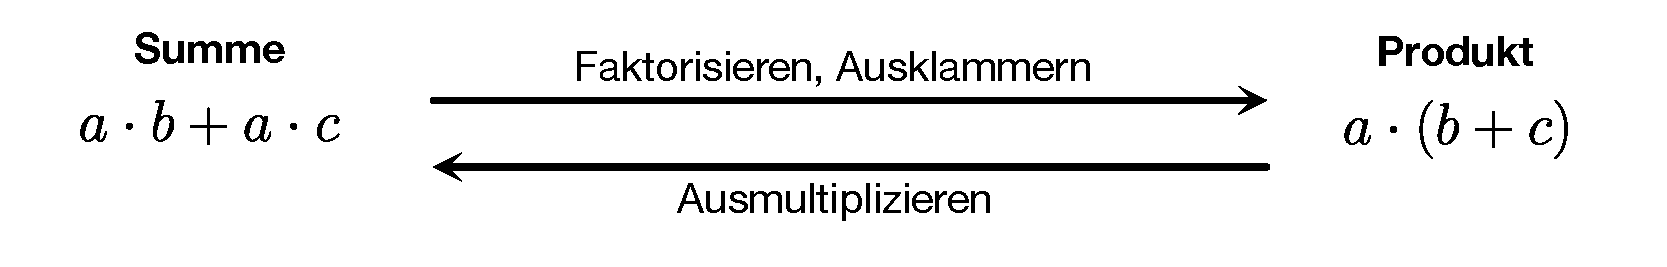
\includegraphics[width=.8\textwidth]{Faktorisieren.pdf}
\end{center}

Das Verwandeln eines Terms von einer Summe zu einem Produkt oder umgekehrt ist eine wichtige grundlegende Umformung, welche wir in der Mathematik immer wieder benötigen werden.

Es gibt ein paar Techniken, mit welchen Terme faktorisiert und ausmultipliziert werden können.

\subsection{Distributivgesetz}

Das Distributivgesetz für die Addition und Multiplikation lautet folgendermassen:
\[
  a\cdot(b+c) = a\cdot b + a\cdot c
\]

Das Distributivgesetz wird angewendet, um gemeinsame Faktoren aus Summanden auszuklammern. Dazu wird der grösste Faktor gesucht, welcher in allen Summanden vorkommt.

\begin{example}
  \textbf{Beispiele:} Faktorisieren Sie den Term $12x+16y$.
  \[
    4(3x+2y)
  \]
  Faktorisieren Sie den Term $4a^{2}+14a$.
  \[
    2a(a+7)
  \]
\end{example}

Auch ganze Terme können Faktoren sein, welche ausgeklammert werden können.

\begin{example}
  \textbf{Beispiel:} Faktorisieren Sie den Term $2(x+2y)-a(x+2y)$.

  Hier kommt der Faktor $(x+2y)$ in beiden Summanden vor und kann ausgeklammert werden:
  \[
    (x+2y)(2-a)
  \]
\end{example}

\subsection{Erste binomische Formel}
\[
  (a+b)^{2} = a^{2} + 2ab + b^{2}
\]
Die erste binomische berechnet die Fläche des Quadrats, das entsteht, wenn das Quadrat mit der Seitenlänge $a$ nach rechts und unten um $b$ vergrössert wird. Dazu wird links und unten ein Rechteck mit der Fläche $ab$ angesetzt. Unten rechts wird noch das Quadrat mit der Seitenlänge $b$ ergänzt.
\begin{center}
  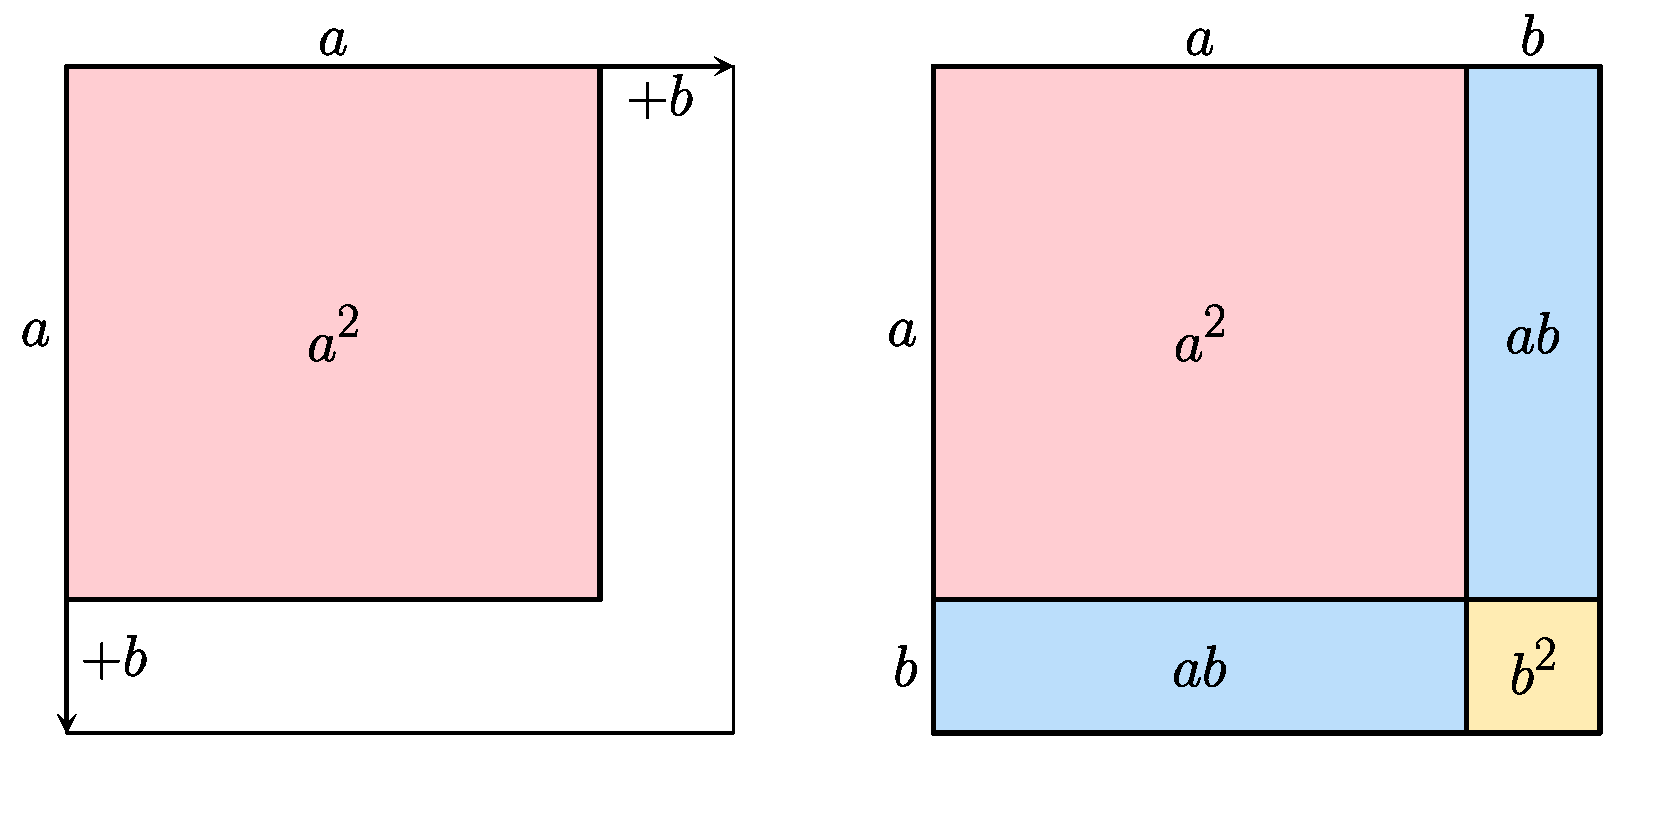
\includegraphics[width=.8\textwidth]{Binomische Formel 1.pdf}
\end{center}
Oft muss ein Term mit Hilfe anderer Regeln umgeformt und vorbereitet werden, bevor er mit einer binomischen Formel faktorisiert werden kann.
\begin{example}
  \textbf{Beispiel:} Faktorisieren Sie den Term $8u^{2}+2z^{2}+8uz$.

  \textbf{Lösung:} Zunächst wird $2$ ausgeklammert (Distributivgesetz):
  \[
    2\left(4u^{2}+z^{2}+4uz\right)
  \]
  Anschliessend werden die Summanden umgestellt (Kommutativgesetz):
  \[
    2\left(4u^{2}+4uz+z^{2}\right)
  \]
  Nun wird im mittleren Summanden der Faktor $2$ separat geschrieben:
  \[
    2\left(4u^{2}+2\cdot 2uz+z^{2}\right)
  \]
  Nun wird die erste binomische Formel angewendet mit $a=2u$ und $b=z$:
  \[
    2(2u+z)^{2}
  \]
\end{example}

\newpage

\subsection{Zweite binomische Formel}
\[
  (a-b)^{2} = a^{2} - 2ab + b^{2}
\]
Die zweite binomische Formel berechnet die Fläche des gelben Quadrats, welches entsteht, wenn vom Quadrat mit der Seitenlänge $a$ seitlich und unten ein Streifen der Breite $b$ abgeschnitten wird. Dabei wird zwei Mal ein Rechteck der Fläche $ab$ abgeschnitten, also $2ab$. Das Quadrat mit der Seitenlänge $b$ wurde dabei jedoch doppelt gezählt. Deshalb muss $b^{2}$ wieder addiert werden.
\begin{center}
  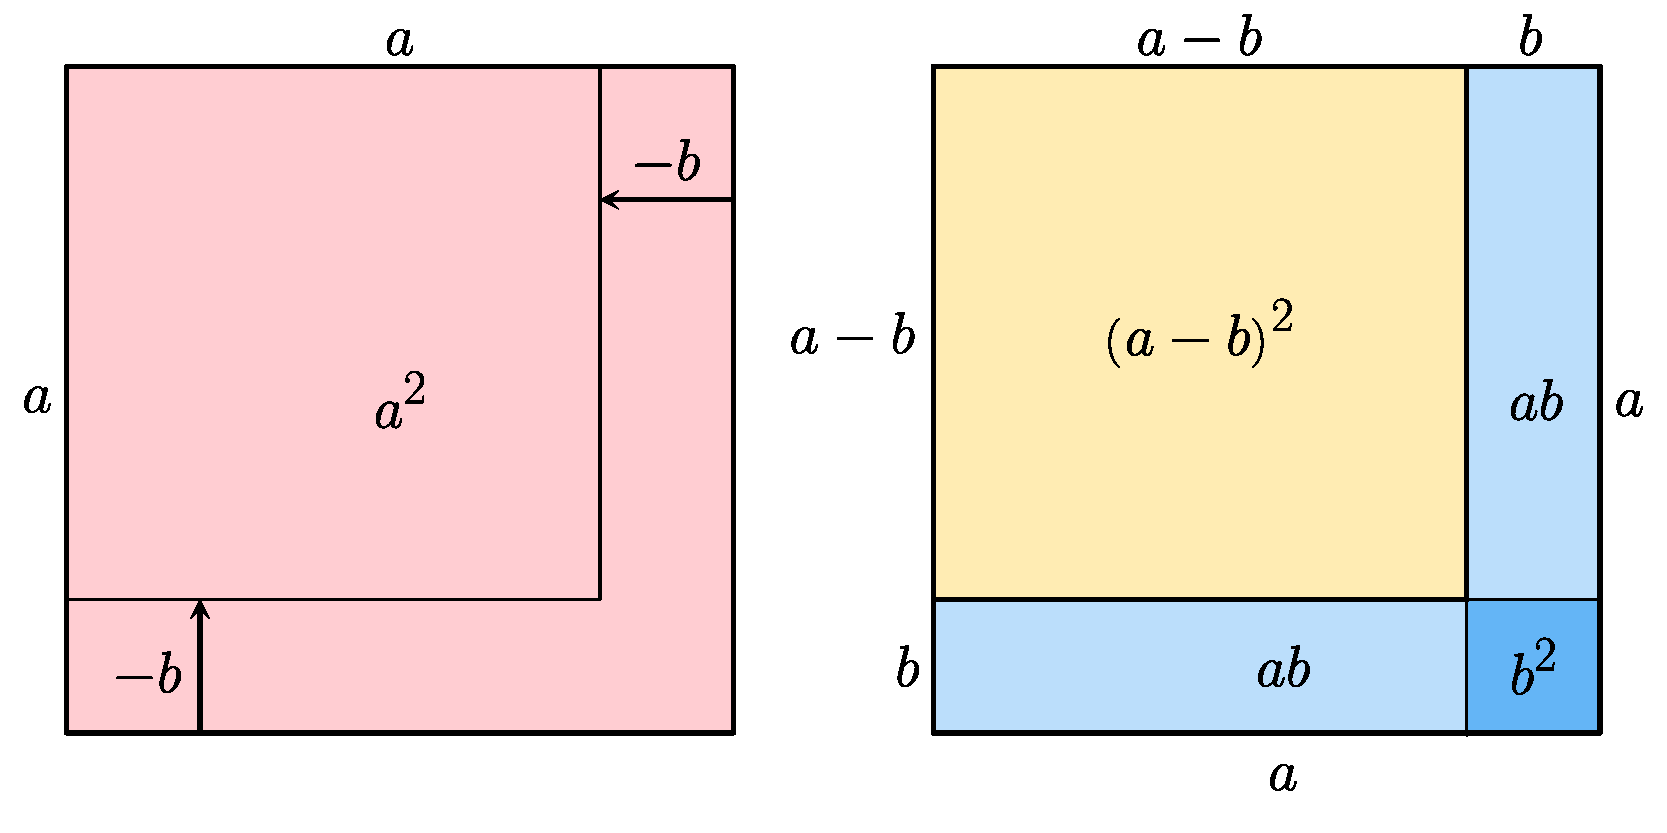
\includegraphics[width=.8\textwidth]{Binomische Formel 2.pdf}
\end{center}

\subsection{Dritte binomische Formel}
\[
  (a+b)(a-b) = a^{2} - b^{2}
\]
Die dritte binomische Formel berechnet die Fläche, welche entsteht, wenn aus dem Quadrat mit der Seitenlänge $a$ ein Quadrat mit der Seitenlänge $b$ ausgeschnitten wird. Die resultierende Fläche kann auseinander geschnitten und so arrangiert werden, dass ein Rechteck mit den Seitenlängen $a+b$ und $a-b$ entsteht.
\begin{center}
  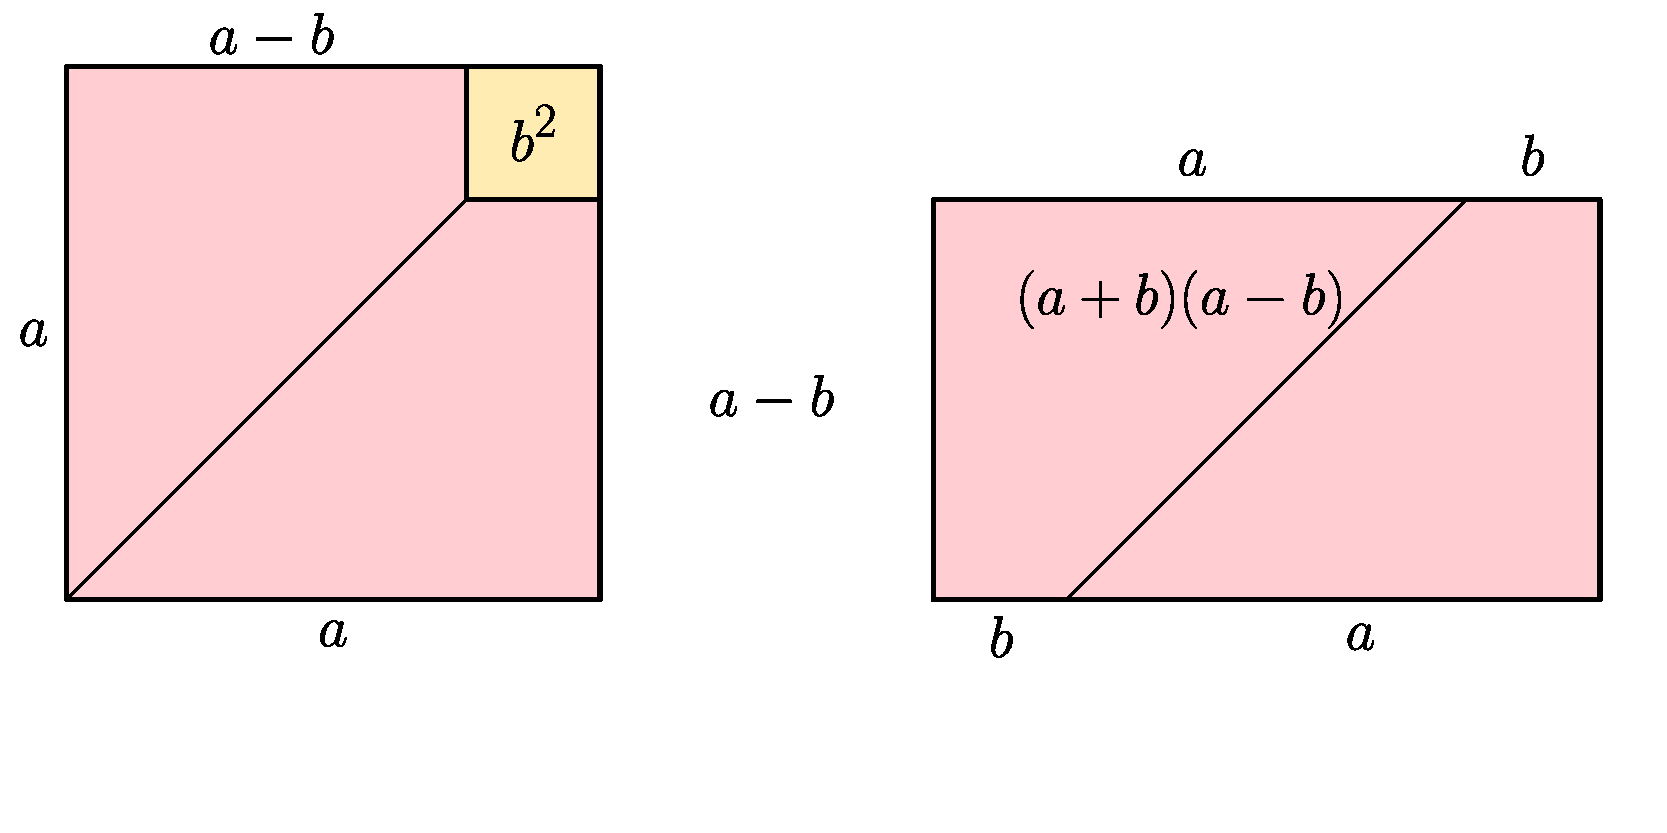
\includegraphics[width=.8\textwidth]{Binomische Formel 3.pdf}
\end{center}

  \newpage
\section{Bruchterme}

% ----------------------------------------------------------------------------
\subsection{Definitionsmenge}
Wenn bei einem Term eine Variable im Nenner vorkommt, so muss durch Angabe der entsprechenden Definitionsmenge sichergestellt werden, dass der Nenner nicht Null werden kann. Dies geschieht am einfachsten, indem die «gefährlichen» Zahlen aus der Grundmenge (normalerweise die reellen Zahlen) ausgeschlossen werden.

Was im Zähler steht, spielt hierbei keine Rolle.
\begin{example}
  \textbf{Beispiele:}
  \begin{align*}
    \frac{1}{a} &\qquad\Rightarrow\qquad \mathbb{D}_{a} = \mathbb{R} \setminus \{0\} &
    \frac{x^{2}}{x-2} &\qquad\Rightarrow\qquad \mathbb{D}_{x} = \mathbb{R} \setminus \{2\} \\[4mm]
    \frac{5z+2}{(z+1)^{2}} &\qquad\Rightarrow\qquad \mathbb{D}_{z} = \mathbb{R} \setminus \{-1\}
  \end{align*}
\end{example}

% ----------------------------------------------------------------------------
\subsection{Kürzen}
Ein Bruchterm darf nur gekürzt werden, wenn sowohl Zähler als auch Nenner als \textbf{Produkt} vorliegen. Wenn in Zähler oder Nenner eine Strichoperation vorkommt, welche nicht in Klammern steht, so ist dies eine Summe und nicht ein Produkt.
\begin{example}
  \textbf{Beispiel:}
  \begin{align*}
    \frac{a+2}{a+3} && \frac{a\cdot 2}{a\cdot 3} = \frac{\cancel{a}\cdot 2}{\cancel{a}\cdot 3}= \frac{2}{3}
  \end{align*}
  Links liegen Summen vor, es darf nicht gekürzt werden, rechts liegen Produkte vor, es kann mit dem Faktor $a$ gekürzt werden.
\end{example}

Um einen Bruchterm zu kürzen, müssen also zunächst Zähler und Nenner in Produkte umgewandelt werden. Dies nennen wir auch \textbf{Faktorisieren}, dazu gibt es ein separates Merkblatt.

\begin{example}
  \textbf{Beispiel:}
  \begin{align*}
    \frac{5a+5}{a^{2}+a} = \frac{5\cdot (a+1)}{a\cdot (a+1)} = \frac{5\cdot \cancel{(a+1)}}{a\cdot \cancel{(a+1)}} = \frac{5}{a}
  \end{align*}
  Hier werden zunächst Zähler und Nenner mit Hilfe des Distributivgesetzes faktorisiert. Anschliessend kann mit dem Faktor $(a+1)$ gekürzt werden.
\end{example}

% ----------------------------------------------------------------------------
\subsection{Multiplizieren}
Bruchterme werden wie Brüche multipliziert, indem die Zähler und Nenner multipliziert werden. Wenn in einem Zähler oder Nenner eine Summe steht, müssen unbedingt Klammern gesetzt werden.
\begin{example}
  \textbf{Beispiel:}
  \begin{align*}
    \frac{x+y}{x-y}\cdot \frac{x}{y} = \frac{(x+y)\cdot x}{(x-y)\cdot y} = \frac{x^{2}+xy}{xy-y^{2}}
  \end{align*}
  Hier werden im letzten Schritt Zähler und Nenner ausmultipliziert. Dies sollte immer nur zuletzt gemacht werden. Wenn noch weiter umgeformt wird, ist es besser, Zähler und Nenner als Produkt beizubehalten.
\end{example}

% ----------------------------------------------------------------------------
\subsection{Addieren}
Bruchterme werden ebenfalls wie Brüche addiert, indem die Nenner gleichnamig gemacht und dann die Zähler addiert werden.
\begin{example}
  \[
    \frac{2}{1-x}+ \frac{3}{x} = \frac{2\cdot x}{(1-x)\cdot x}+\frac{3\cdot (1-x)}{x\cdot (1-x)} = \frac{2x+3-3x}{(1-x)x} = \frac{5x+3}{(1-x)x}
  \]
\end{example}

\end{document}
